\documentclass[10pt,twocolumn]{article}
	
\usepackage{myfontstyle}
\usepackage{mypackages}
\usepackage{mymacros}
\usepackage{mycommands}

\begin{document}
\thispagestyle{fancy1}

%%% Title and Abstract------------------------
\twocolumn[
\begin{center}
	\hrule
	\vspace{3pt}
	% Title:
	{\sffamily\bfseries\Large
		Report for Laboratory 2: Voltage Dividers
	} \\
	{\color{gray}
		\vspace{3pt}
		\hrule
		\vspace{3pt}
	}
	{
		\hspace*{\fill}
		Austin Piper
		\hspace*{\fill}
		Alex Blakely
		\hspace*{\fill}
		Ahmed Irfan
		\hspace*{\fill}
%		Fourth Author    % uncomment these two lines if there's a fourth author
%		\hspace*{\fill}
	}\\
	\vspace{3pt}
	{\itshape
		\hspace*{\fill}
		Department of Mechanical Engineering, Saint Martin's University
		\hspace*{\fill} \\
		\hspace*{\fill}
		ME/EE 316---Mechatronics \& Measurements Laboratory
		\hspace*{\fill}
	}\\
	\vspace{3pt}
	{
		\hspace*{\fill}
		\today{} % today's date ... can type manually instead
		\hspace*{\fill}
	}
	\vspace{3pt}
	{\color{gray}\hrule}
%	\vspace{2pt}
\end{center}
% Abstract:
\begin{adjustwidth}{1.5in}{1.5in}
{\small
\noindent\textbf{Abstract.} \hspace{1em}
	Applying a 10V power supply to a voltage divider circuit with two resistors in series the voltage across both resistors is constant, although voltage across a single resistor is changing depending on resistance. Using a myRiO configured with the labVIEW software to change our input voltage and measure the voltage source and the resistor voltage. Connecting a function generator to an oscilloscope, a variety of functions at 5Vpp had a period of 2.5ms.
}
\end{adjustwidth} 
\vspace{9pt}
\hrule
\vspace{1\baselineskip}
]

%%% Body -------------------------


\section{Introduction} 
\label{sec:introduction}

``Introduce what your question is. Explain why someone should find this interesting. Summarize what is currently known about the question. Introduce a little of what you found and how you found it. You should explain any ideas or techniques that are necessary for someone to understand your results section.''

Typically, you will be asked to include in your report a theoretical prediction for comparison with your experimental results. Typically, this section is a good place for presenting that. You needn't always include every aspect of your derivation, but you should "sketch out" the process, hitting the "highlight" ideas an equations along the way. Typically there's no need to, say, plot the results here, since you'll be plotting them again alongside the data in the Results section (\autoref{sec:results}). 

\section{Materials and Methods}

``This is like a cooking recipe. Include enough detail so that someone can repeat the experiment. It is important that the reader be able to interpret the results knowing the context in which they were obtained.

``The Materials and Methods section should be written in the past tense, since your experiments are completed at the time you are writing your paper.''

Here are some things you don't want to do in this section.

\begin{enumerate}
\item 
Don't simply copy and paste material from my description. 
\item 
Don't simply list the procedure in bullet points (although some lists are fine). I want a description in \emph{your} words.
\item
Don't use a figure from my description unless you properly cite it! A proper citation would be \citep[p.~32]{Picone2018}.
\end{enumerate}

\section{Results}
\label{sec:results}

``To write the results section, use the figures and tables as a guide. Start by outlining, in point form, what you found, going slowly through each part of the figures. Then take the points and group them into paragraphs, and finally order the points within each paragraph. Present the data as fully as possible, including stuff that at the moment does not quite make sense.

``Verbs in the results section are usually in the past tense. Only established scientific knowledge is written about in the present tense, `the world is round,' for example. You cannot presume that your own data are part of the body of established scientific knowledge, and so when you describe your own results, use the past tense, `a band of 1.3 KB was seen,' for example. There are, however, exceptions to this general rule. It is acceptable to say, `Table 3 shows the sizes of the DNA fragments in our preparation.' It is also acceptable to say, `In a 1991 paper, Ebright and coworkers used PCR to mutagenize DNA.' \ldots

``Some readers begin by scanning the figures first. The figures, with the legends, should provide a self-explanatory overview of your data. Decide what the data show, then create figures which highlight the most important points of your paper.

``Tables are used to present repetitive data that is numerical. Graphs or illustrations, collectively called figures, are used to present numerical trends, raw data (like a picture of a gel), or a model that explains your work.

``When you prepare your figures and tables, keep in mind that it is significantly more expensive for journals to publish figures and tables than text, so try to present the data in a way that is worthy of such added expense.''

\section{Discussion}

``This is the section of the paper for you to show off your understanding of the data. You should summarize what you found. Explain how this relates to what others have found. Explain the implications.''

\section{Author Contributions}

You are required to describe each member's contributions to the laboratory exercise and report.

%%% References -------------------------

\bibliographystyle{plainnat}
\bibliography{report}

%%% Appendices -------------------------

\appendix

\section{Appendix: \LaTeX{} Tutorial}\label{sec:latex}

I'm going to teach you how to use \LaTeX{} a little bit. Like how to cite a source, insert a graphic, and build tables. Follow along in the \texttt{report.tex} file.

{\bfseries\color{red} Do not use this appendix as any sort of template for the report! Equations, figures, and tables should appear in the body of the report.} Delete this appendix before submitting your report.

\subsection{Citing a Source}

Let's cite a source. The source must be already saved as a BibTeX file (\texttt{.bib}) in the same directory as the \texttt{.tex} document. I have already created a sample \texttt{report.bib} file. (If you want to add and remove sources to this file, you may use a reference manager like BibDesk on a Mac or JabRef on a PC.)

The next step is to cite the source, inline~\citep{Rowell1997}. And I can easily cite another reference~\citep{Ciesielski1997}.

\subsection{Equations}

Equations should appear in the body of the report, especially in the Introduction (\autoref{sec:introduction}), when describing your theoretical predictions. An equation should be part of a complete sentence.

Here are some examples.

We now see that
\begin{align}
	x = 1 .
\end{align}

Somehow, the following impossible equation hold:
\begin{align} \label{eq:int}
	\int_0^t x_2 \sin{x} dx = 
	\begin{bmatrix}
		1 & 0 & 8 \\
		0 & x^7 \\
		7 &
	\end{bmatrix} .
\end{align}
We now see that 
\begin{align}
	\bm{x} = \bm{\alpha} 
    \left( 
    	\left(
        	\frac{2}{3}
        \right) + 
        \frac{5}{6} 
    \right) , 
\end{align}
where $\bm{\alpha}$ is the coefficient of stupidity.

And this works too: $\frac{\partial x}{\partial y}$ .

\begin{subequations}
\begin{align*}
	x &= 2 y & \text{(where $x>2$)} \\
	y &= 4 x + 8 &
\end{align*}
\end{subequations}

Later, you could refer to the equation \autoref{eq:int}.

Or you could do it multiple times: \autoref{eq:int}.

\subsection{Figures}
It is easy enough to add a figure. In the subdirectory \texttt{figures}, I placed a file \texttt{data.pdf}. If we want to include it in the document, we use the following commands.

\begin{figure}[bt]
	\centering
	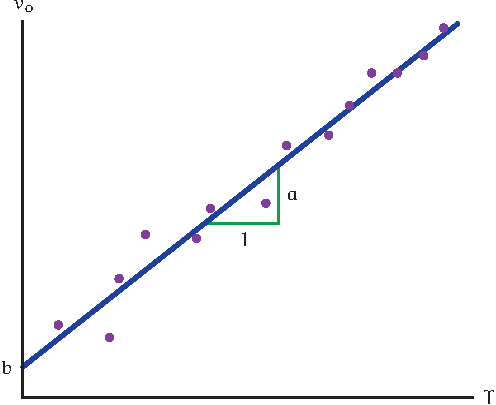
\includegraphics[width=.9\linewidth]{figures/data.pdf}
	\caption{here's a caption.}
	\label{fig:data}
\end{figure}

We can easily reference the figure with its label, like \autoref{fig:data}.

\subsection{Tables}
Tables can be a pain in \LaTeX{}. Here's a simple table.

Notice (as in \autoref{tab:dummy}) that these things don't go where they're entered. Most of the time it's preferable to have a figure or table ``float'' such that it is at the top or bottom of a column.
 
\begin{table}[bt]
	\begin{tabularx}{1\linewidth}{ lXX }
		\hline
		 & \textbf{label 1} & \textbf{label 2} \\
		\hline
		Interesting thing & $5.1$ & $603$ \\
		Thing of interest & pigtails & $x^3$ \\
		\hline
	\end{tabularx}
	\caption{a table caption.}
	\label{tab:dummy}
\end{table}


\end{document}  